\documentclass[11pt,a4paper,titlepage,oneside]{report}

%%% RELACIÓN DE VARIABLES A PERSONALIZAR %%%
% \def\lingua{gal}
\def\lingua{esp} % descomenta esta liña se redactarás a memoria en español
%\def\lingua{eng} % descomenta esta liña se redactarás a memoria en inglés
\def\nome{David Rodríguez Bacelar}                             % substitúe aquí o teu nome
\def\nomedirectorA{Patricia Martín Rodilla, David Otero Freijeiro}              % substitúe aquí o nome de quen dirixe
%\def\nomedirectorB{Outro Nome Completo}             % duplica esta liña máis veces se o precisas, cambiando
% a letra final (A, B, C, D...): úsanse na portada.tex
\def\titulo{Perfilado automático de usuarios en corpus sociales sobre el movimiento Black Lives Matter} % substitúe aquí o título do teu TFG
%\def\titulacion{gced}                               % descomenta esta liña e comenta a seguinte se es estudante do GCED
\def\titulacion{gei}
\def\mencion{COMPUTACIÓN}
% \def\mencion{ENXEÑARÍA DO SOFTWARE}
%\def\mencion{ENXEÑARÍA DE COMPUTADORES}
%\def\mencion{SISTEMAS DE INFORMACIÓN}
%\def\mencion{TECNOLOXÍAS DA INFORMACIÓN}

\def\renomearcadros{si}

\usepackage{estilo_tfg}

% Lista de paquetes potencialmente interesantes (uso baixo demanda)

\usepackage{fancyvrb}
\fvset{xleftmargin=1em,frame=single,fontsize=\small,numbers=left}
\usepackage{pgfplots}
\pgfplotsset{width=10cm,compat=1.9}
\usepackage[edges]{forest}
\tikzset{element/.style={align=center,text width=2cm,rounded corners=6pt}}
\usetikzlibrary{intersections,backgrounds}
% \usepgfplotslibrary{external}
% \tikzexternalize
% \usepackage{alltt}       % proporciona o entorno alltt, semellante a verbatim pero que respecta comandos
% \usepackage{enumitem}    % permite personalizar os entornos de lista
% \usepackage{eurofont}    % proporciona o comando \euro
\usepackage{float}       % permite máis opcións para controlar obxectos flotantes (táboas, figuras)
% \usepackage{hhline}      % permite personalizar as liñas horizontais en arrays e táboas
\usepackage{longtable}   % permite construir táboas que ocupan máis dunha páxina
% \usepackage{lscape}      % permite colocar partes do documento en orientación apaisada
% \usepackage{moreverb}    % permite personalizar o entorno verbatim
% \usepackage{multirow}    % permite crear celdas que ocupan varias filas da mesma táboa
% \usepackage{pdfpages}    % permite insertar ficheiros en PDF no documento
% \usepackage{rotating}    % permite diferentes tipos de rotacións para figuras e táboas
\usepackage{subcaption}
\usepackage{hhline}
% \usepackage{tabu}        % permite táboas flexibles
% \usepackage{tabularx}    % permite táboas con columnas de anchura determinada
\colorlet{punct}{red!60!black}
\definecolor{background}{HTML}{EEEEEE}
\definecolor{delim}{RGB}{20,105,176}
\colorlet{numb}{magenta!60!black}

\usepackage{sourcecodepro}

\lstdefinelanguage{json}{
    basicstyle=\scriptsize\ttfamily,
    numbers=left,
    numberstyle=\tiny,
    stepnumber=1,
    numbersep=4pt,
    showstringspaces=false,
    breaklines=true,
    frame=none,
    backgroundcolor=\color{background},
    literate=
     *{0}{{{\color{numb}0}}}{1}
      {1}{{{\color{numb}1}}}{1}
      {2}{{{\color{numb}2}}}{1}
      {3}{{{\color{numb}3}}}{1}
      {4}{{{\color{numb}4}}}{1}
      {5}{{{\color{numb}5}}}{1}
      {6}{{{\color{numb}6}}}{1}
      {7}{{{\color{numb}7}}}{1}
      {8}{{{\color{numb}8}}}{1}
      {9}{{{\color{numb}9}}}{1}
      {:}{{{\color{punct}{:}}}}{1}
      {,}{{{\color{punct}{,}}}}{1}
      {\{}{{{\color{delim}{\{}}}}{1}
      {\}}{{{\color{delim}{\}}}}}{1}
      {[}{{{\color{delim}{[}}}}{1}
      {]}{{{\color{delim}{]}}}}{1},
}

\pgfplotsset{
  y tick label style={
    /pgf/number format/.cd,%
    scaled y ticks=false,
    set thousands separator={.},
    set decimal separator={,},
    fixed,
  },
  x tick label style={/pgf/number format/set thousands separator={}},
  tick label style={
    font=\scriptsize
  },
  nodes near coords,
  every node near coord/.append style={
    font=\tiny
  },
  every node near coord/.append style={
    /pgf/number format/.cd,%
    set thousands separator={.},
    set decimal separator={,},
    fixed,
    /tikz/.cd
  },
}

%%%%%%%%%%%%%%%%%%%%%%%%%%%%%%%%%%%%%%%%%%%%%%%%%%%%%%%%%%%%%%%%%%%%%%%%%%%%%%%%
% Corpo                                                                        %
%%%%%%%%%%%%%%%%%%%%%%%%%%%%%%%%%%%%%%%%%%%%%%%%%%%%%%%%%%%%%%%%%%%%%%%%%%%%%%%%

\begin{document}

\setlength\arrayrulewidth{0.7pt}

%%%%%%%%%%%%%%%%%%%%%%%%%%%%%%%%%%%%%%%%
% Preliminares do documento            %
%%%%%%%%%%%%%%%%%%%%%%%%%%%%%%%%%%%%%%%%

\begin{titlepage}
  
  \hspace*{128pt}
  \textcolor{udcpink}{{\fontencoding{T1}\fontfamily{phv}\selectfont Facultade de Informática}}\\[-32pt]

  \begin{center}
    
\includegraphics[scale=0.3]{imaxes/udc}\\[25pt]

    {\large TRABALLO FIN DE GRAO \\
            \nometitulacion \\
            \nomemencion } \\[10pt]

    \carimbo \\[25pt]

    \begin{huge}
      \begin{spacing}{1.3}
        \bfseries \titulo
      \end{spacing}
    \end{huge}
  \end{center}
  
  \vfill
  
  \begin{flushright}
    {\large
    \begin{tabular}{ll}
      {\bf Estudante:} & \nome \\
      {\bf Dirección:} & \nomedirectorA \\
%                      & \nomedirectorB \\ % duplica esta liña máis veces se o precisas, cambiando
                                           % a letra final (A, B, C, D...); define eses nomes no memoria_tfg.tex
    \end{tabular}}
  \end{flushright}
  \rightline{A Coruña, \datasimple.}
\end{titlepage}

\dedicatoria{A todos los que me ayudaron a llegar hasta aquí.}
\paxinaenbranco\
\begin{agradecementos}
  En primer lugar, me gustaría agradecerles a mis tutores, Patricia y David, por su ayuda durante todo el desarrollo del trabajo y por sentar
  las bases de lo que es este proyecto.

  Agradecerle a mi familia por su incansable paciencia, su constante apoyo y sus incontables
  palabras de ánimo durante todo este tiempo, sin las cuales todo habría sido mucho más difícil.

  Quería agradecerle también a mi pareja todo lo que me da día a día, todo el apoyo que hace que pueda
  seguir adelante ante cualquier problema y todo lo que significa para mí una persona tan maravillosa
  en todos los sentidos y sin la que no habría llegado a ser quien soy.

  Por úlitmo, agradecerles a todos mis amigos, tanto a los que tuve la oportunidad de conocer durante
  la carrera como a los de toda la vida, haciendo mención especial a mi gran amigo y compañero de
  piso, por todo lo que me ha aportado desde que lo conocí.
\end{agradecementos}
%%%%%%%%%%%%%%%%%%%%%%%%%%%%%%%%%%%%%%%%%%%%%%%%%%%%%%%%%%%%%%%%%%%%%%%%%%%%%%%%

\pagestyle{empty}
\begin{abstract}
  Con el objetivo de proporcionar una herramienta útil basada en el perfilado automático de autores, a lo largo de este trabajo
  se profundizará más en este campo en el contexto de las redes sociales, analizando cuáles son los mejores algoritmos,
  las técnicas más utilizadas y las características más comúnes que se suelen emplear.
  Asimismo, se desarrollará, bajo la metodología SCRUM, una aplicación web en la que se permita a los usuarios perfilar los autores de una
  colección de textos propia —haciendo uso de algoritmos seleccionados en la fase previa de investigación— y mostrando los resultado del perfilado en un \textit{dashboard} intuitivo y accesible.
  Finalmente, para mostrar un caso de uso real de la aplicación se empleará la colección de referencia sobre el movimiento \textit{Black Lives Matter} (\#BLM),
  puesta a disposición para este TFG por los tutores del mismo, con el objetivo de analizar el perfil de los usuarios que participaron en los debates en las redes sociales sobre este movimiento
  de gran relevancia social.

  \vspace*{25pt}
  \begin{segundoresumo}
    To provide a useful tool based on automatic author profiling, throughout this work, will research deeper into this field in the context of social networks, analyzing the best algorithms,
    the most commonly used techniques, the most commonly used techniques, and the typical features that are often employed. Furthermore, under the SCRUM methodology, we will
    develop a web application, allowing users
    to profile authors of their own text datasets employing algorithms selected in the previous research phase— and displaying the profiling results on an intuitive and accessible dashboard.
    Finally, to illustrate a real use case of the application, the reference collection related to the "Black Lives Matter" movement (\#BLM) will be utilized. This collection has been made available for
    this Bachelor's Thesis by its supervisors, with the aim of analyzing the profiles of users who participated in social media discussions about this socially significant movement.
  \end{segundoresumo}
  \vspace*{25pt}
  \newpage
\begin{multicols}{2}
\begin{description}
\item [\palabraschaveprincipal:] \mbox{} \\[-20pt]
  \begin{itemize}
    \item \textit{Perfilado de autor}
    \item \textit{Redes sociales}
    \item \textit{Procesado de lenguaje natural}
    \item \textit{Aplicación web}
    \item \textit{Aprendizaje automático}
  \end{itemize}
\end{description}

\begin{description}
\item [\palabraschavesecundaria:] \mbox{} \\[-20pt]
  \begin{itemize}
    \item \textit{Author profiling}
    \item \textit{Social networks}
    \item \textit{Natural language processing}
    \item \textit{Web application}
    \item \textit{Machine learning}
  \end{itemize}
\end{description}
\end{multicols}

\end{abstract}
\pagestyle{fancy}

%%%%%%%%%%%%%%%%%%%%%%%%%%%%%%%%%%%%%%%%%%%%%%%%%%%%%%%%%%%%%%%%%%%%%%%%%%%%%%%%


\pagenumbering{roman}
\setcounter{page}{1}
\bstctlcite{IEEEexample:BSTcontrol}

\tableofcontents
\listoffigures
\listoftables
\clearpage

\pagenumbering{arabic}
\setcounter{page}{1}

%%%%%%%%%%%%%%%%%%%%%%%%%%%%%%%%%%%%%%%%
% Capítulos                            %
%%%%%%%%%%%%%%%%%%%%%%%%%%%%%%%%%%%%%%%%

\chapter{Introducción}
\label{chap:introduccion}

\lettrine{A}{partir} de la segunda década de los 2000, las redes sociales han experimentado
un crecimiento continuado de su uso, tanto en número de usuarios como en
cantidad de información generada. Como se muestra en el informe \textit{Digital 2023 Global Overview Report} (We Are Social et al., 2023)
\cite{wearesocial}, a principios del año 2013 existían alrededor de 1.700 millones de usuarios en las redes sociales,
mientras que a principios del año 2023, esta cifra aumentó hasta los 4.700 millones, con una variación anual media del 10,8\% (se puede ver
más información en la Figura \ref{fig:usuarios_redes_sociales}).
Así, plataformas como Facebook, Instagram, Twitter o YouTube, cuentan con millones de usuarios activos diariamente,
donde se comparte información o se crea contenido de entretenimiento. Además, las redes sociales se han convertido en
un lugar donde se debate sobre temas políticos, sociales o económicos, y donde se comparten diversas opiniones y noticias.
Este hecho se puede ver, de nuevo, en el informe mencionado anteriormente, donde se muestra que el 34,2\% de los usuarios
de redes sociales las utilizan para informarse sobre noticias, el 28,8\% para saber cuáles son los temas de actualidad
y el 23,4\% para compartir opiniones y debatir con otros usuarios.

\bigskip
\begin{figure}[H]
	\centering
	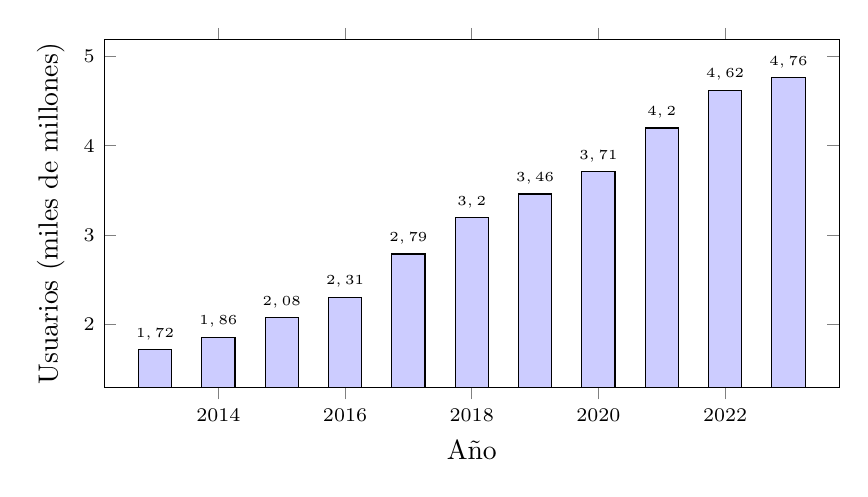
\begin{tikzpicture}
		\begin{axis}[
				width=0.9\textwidth,
				height=6cm,
				xmajorgrids=false,
				ylabel=Usuarios (miles de millones),
				xlabel=Año,
				ybar=6pt,
				bar width=12pt,
				enlarge x limits=0.08,
				enlarge y limits=0.14,
			]
			\addplot[fill=blue!20]
			coordinates {(2013,1.720) (2014,1.857) (2015,2.078)
					(2016,2.307) (2017,2.789) (2018,3.196) (2019,3.461)
					(2020,3.709) (2021,4.199) (2022,4.623) (2023,4.760)};
		\end{axis}
	\end{tikzpicture}
	\caption{Evolución del número de usuarios en redes sociales}
	\label{fig:usuarios_redes_sociales}
\end{figure}

\section{Importancia de las redes sociales}
\label{sec:intr_importancia}
Toda esta información generada tiene una gran relevancia a distintos niveles. En primer lugar, cabe destacar el impacto que
tienen las redes sociales a nivel político. Y es que en la actualidad, vivimos en una campaña permanente (Blumenthal, 1980)
\cite{sydney1980permanent},
donde el acceso a estas plataformas ofrece la posibilidad a los ciudadanos de estar informados sobre política, mientras que a las instituciones
de poder les permite conocer el estado de la opinión pública (Strömbäck, 2008)
\cite{stromback2008four}, pudiendo llegar a influenciar "mucho" o "bastante" la intención de voto (Gallardo-Paúls, 2016) \cite{gallardo2016pseudopolitica}.
En segundo lugar, el contenido que se genera en las redes sociales es de gran relevancia a nivel sociológico ya que sirve para analizar, entre muchas cosas,
la representación que tienen en ellas la sociedad o la forma en la que interactuamos (Mislove et al., 2011) \cite{mislove2011understanding}. Cabe resaltar también la influencia
que tienen las plataformas digitales a nivel económico, ya que se han convertido en un lugar donde las empresas
publicitan sus productos y servicios y a las que destinan gran parte de sus presupuestos en publicidad
(Saxena et al., 2013) \cite{saxena2013advertising}. Finalmente, destacar el rol fundamental que juega la seguridad en las redes sociales,
ya que se han convertido en lugares donde se comparte información personal, y donde se pueden cometer delitos como
el \textit{cyberbullying} o el \textit{grooming} (Machimbarrena et al., 2018) \cite{machimbarrena2018internet}.

\section{Perfilado de autor}
\label{sec:intro_perfilado}

El perfilado de autor, también conocido como perfilado de usuario o \textit{author profiling} en inglés, consiste en determinar, a partir de un texto,
las características de su autor, como su género, edad, rasgos personales, etc. Para ello se hace uso de diversas técnicas de aprendizaje automático
basadas en el procesado del lenguaje natural (\textit{Natural Language Processing} o NLP en inglés), que permiten extraer características lingüísticas del texto y utilizarlas para una
posterior clasificación.

\bigskip
De esta forma, el perfilado de autor en redes sociales se ha convertido en un área de investigación de gran interés
en los últimos años, posicionándose como una herramienta de creciente importancia en campos como la seguridad, el \textit{marketing}
o la investigación forense (Rangel et al., 2013) \cite{rangel2013overview}. Así, la evolución y el perfeccionamiento del perfilado de autor propiciaría la creación de
una herramienta de gran ayuda para los sociólogos a la hora de realizar análisis sobre temas que dispongan de información digital;
ofrecería a las empresas  una forma de conocer el perfil de los clientes que opinan de
forma positiva y negativa de sus productos; tendría un gran valor
para los partidos políticos, dado que podrían conocer cuál es el perfil de sus votantes; y respaldaría el trabajo de los cuerpos de seguridad
a la hora de la evaluación de sospechosos en base a su perfil lingüístico.

\section{Objetivos del trabajo}
\label{sec:intro_objetivos}

Tras la introducción al perfilado de autor y las motivaciones que existen para su estudio a nivel de las redes sociales,
se expondrán a continuación los objetivos principales de este trabajo.

\bigskip
El primero de ellos es la investigación del estado del arte del perfilado automático de autor, enmarcado en
el análisis de documentos digitales. Para acotar
el estudio, la investigación se centrará en el perfilado de autor en el ámbito de la lengua inglesa y se priorizarán
aquellos algoritmos que perfilen los rasgos generacionales del autor.
Asimismo, se profundizará en cuáles son las técnicas de aprendizaje automático más utilizadas en el campo,
cuáles son las características que se extraen comúnmente y cuáles son los algoritmos que mejores resultados obtienen.

\bigskip
Como segundo objetivo, una vez se hayan logrado ejecutar satisfactoriamente los algoritmos seleccionados tras el estudio,
se pretende desarrollar una aplicación que permita a los usuarios el perfilado automático de una serie de características
demográficas de una colección de textos, mostrando un tablero web visual de datos (\textit{dashboard} en inglés) accesible y usable con los resultados obtenidos.
Además, se liberará el código de la aplicación en un repositorio público de GitHub \cite{github}, para que pueda ser utilizado de forma
gratuita por cualquier persona y pueda crecer gracias a la colaboración de la comunidad.

\bigskip
Por último, empleando la aplicación previamente desarrollada, se utilizará como caso de uso la colección sobre el movimiento
\textit{Black Lives Matter} (\#BLM) proporcionada para este TFG. Se busca, por lo tanto, realizar un análisis con un componente sociológico
de los perfiles obtenidos,
con el objetivo de obtener conclusiones acerca del movimiento y de los usuarios que participaron debatiendo sobre el mismo en las redes sociales.

\bigskip
Se trata, en definitiva, de un trabajo que pretende profundizar en el perfilado de autor, tanto desde un punto de vista teórico como práctico,
haciendo accesible mediante la creación de una aplicación, una herramienta basada en técnicas de aprendizaje automático, y
demostrando su utilidad con el análisis de un fenómeno social de gran relevancia.

\section{Estructura de la memoria}
\label{sec:intro_estructura}

La memoria se estructura en diez capítulos que se describen a continuación:

\begin{itemize}
	\item \textbf{Introducción}: Se trata del capítulo actual; en él se contextualiza el perfilado automático de autores junto a su utilidad
	      para el análisis de la información generada en las redes sociales. Asimismo, se exponen los objetivos que tiene este trabajo y la estructura
	      de esta memoria.

	\item \textbf{Estado del arte del perfilado de autor}: En este capítulo se realiza una revisión bibliográfica desde los inicios del perfilado de autor y se explican
	      los conceptos básicos que se utilizan habitualmente en el campo. Posteriormente, se analizan las tareas sobre el perfilado de autor celebradas,
	      seleccionando y evaluando diferentes algoritmos presentados en las mismas.

	\item \textbf{Herramientas, técnicas y lenguajes}: Tercer capítulo de la memoria, donde se exponen las herramientas utilizadas en todo el proceso de desarsrollo
	      y se argumenta la elección de cada una de ellas.

	\item \textbf{Metodología}: En este capítulo se explica la metodología que se ha seguido para el desarrollo de la aplicación, así como
	      los roles que desempeña cada uno de los miembros del equipo junto a las adaptaciones que se han realizado a la metodología propuesta.

	\item \textbf{Análisis}: A lo largo de este capítulo se detallan los requisitos funcionales y no funcionales identificados para la aplicación.

	\item \textbf{Diseño}: En este capítulo se muestran los diagramas de arquitectura y de clases diseñados, así como los prototipos de la interfaz web de usuario.

	\item \textbf{Implementación}: Séptimo capítulo de la memoria; en él se explica a bajo nivel las adaptaciones que fueron necesarias para integrar los algoritmos
	      seleccionados en la aplicación. Además, se detalla la estructura de directorios del proyecto y se justifica la decisión de liberar el código fuente.

	\item \textbf{Caso de uso \#BLM}: En este capítulo se utiliza como ejemplo de caso de uso de la aplicación el análisis de la colección de referencia ofrecida para este TFG
	      sobre el movimiento \textit{Black Lives Matter}.

	\item \textbf{Planificación y costes}: A lo largo de este capítulo se explican las tareas realizadas en cada \textit{sprint} y se desglosan los costes
	      económicos derivados del proyecto.

	\item \textbf{Conclusiones}: Capítulo final de la memoria, en el que se exponen las líneas de trabajo futuras y se realiza una valoración de los conocimientos
	      adquiridos durante todo el proceso.

\end{itemize}

\chapter{Estado del arte del perfilado de autor}
\label{chap:estadoarte}

Durante los inicios del perfilado automático de autor, los algoritmos se centraban en la tarea de la clasificación por género.
En esta línea, trabajos como (Koppel et al., 2002)\cite{koppel2002automatically} se desmarcaban de la tendencia de la época,
la cual se basaba en la clasificación de textos en base a su contenido, para centrarse en la clasificación de textos \textbf{en base a su estilo}. En este caso, se centraban en la obtención del género del autor mediante el análisis
de 920 documentos de carácter formal escritos en inglés con una media de alrededor de 34.300 palabras cada uno, obteniendo una precisión en la clasificación de
aproximadamente el 77\%.

\bigskip
Así, la demostración de la existencia de rasgos diferenciadores en la escritura que permitían perfilar ciertos ascpectos del individuo, especialmente del género, 
supuso un gran avance en el campo del perfilado de autor
y dió pié a la realización de trabajos como (Argamon et al., 2003)\cite{argamon2003gender}, (Corney et.al, 2002)\cite{corney2002gender} o (Otterbacher et al., 2010)\cite{otterbacher2010inferring}, 
así como también permitió el inicio de una clasificación más compleja en base a otras características como la edad, la orientación sexual o la personalidad.

\bigskip
Más tarde, en el año 2011 se celebraría el primer evento organizado por el \textit{PAN} (\textit{Plagiarism Analysis, Authorship Identification, and Near-Duplicate Detection}) \cite{pan},
un foro de investigación que organiza eventos científicos y tareas anuales relacionadas con el análisis forense de textos digitales
y rasgos estilométricos. La primera de estas tareas centrada en el perfilado de autor se celebraría en el año 2013 (Rangel et al., 2013)\cite{rangel2013overview},
en la que se pedía a los participantes que obtuvieran, a partir de una serie de \textit{tweets}, la edad y el género de su autor. El ganador de este concurso obtuvo una
precisión del 60\% en la clasificación de género y del 67\% en la clasificación de edad, haciendo uso, la mayor parte de los participantes, de técnicas de aprendizaje
supervisado como los Árboles de Decisión (en inglés \textit{Decission Trees}) o las Máquinas de Soporte Vectorial (en inglés \textit{Support Vector Machines}) e inluyendo
en sus modelos características basadas en el TF-IDF, n-gramas, etiquetas POS o características como el número de emoticonos o la frecuencia de signos de puntuación.
En los siguientes años se celebrarían nuevas ediciones de esta tarea (Rangel et al., 2014\cite{rangel2014overview}, Rangel et al., 2015\cite{rangel2015overview},
Rangel et al., 2016\cite{rangel2016overview}...), añadiendo nuevas sub-tareas como el reconocimiento de rasgos personales, la ocupación o los dialectos del lenguaje,
así como también alcanzando mejores resultados en la clasificación.

\section{Algoritmos analizados}
\label{sec:algoritmos_analizados}

TODO
% Todos estos algoritmos se basan en lo que en recuperación de información se conoce como \textit{TF-IDF} (del inglés \textit{Term Frequency-Inverse Document Frequency}), 
% que es una medida numérica que expresa cuán relevante es una palabra para un documento en una colección. 
% La importancia aumenta proporcionalmente al número de veces que una palabra aparece en el documento, pero se compensa con la frecuencia 
% de la palabra en la colección de documentos, lo que permite manejar el hecho de que algunas palabras son generalmente 
% más comunes que otras.

\chapter{Herramientas, técnicas y lenguajes}
\label{chap:herramientas}

A lo largo de este capítulo se describirán las herramientas utilizadas para el desarrollo del proyecto y se expondrán las
razones de su uso. A su vez, para una mejor estructuración, dividiremos dichas herramientas en cuatro grupos diferentes:
\textit{frontend}, \textit{backend}, algoritmos de perfilado y herramientas de soporte.
	
\section{\textit{Backend}}
\label{sec:herramientas_backend}

Ya que para el \textit{backend} no se necesitaba nada excesivamente complejo, se decidió utilizar el lenguaje de programación Python \cite{python} junto
con el \textit{framework} FastAPI \cite{fastapi}, el cual permite crear APIs REST de forma sencilla. La decisión de utilizar Python, viene
condicionada por el hecho de que los algoritmos de perfilado de autor utilizados, así como también la mayor parte de los algoritmos de aprendizaje automático
y procesamiento de lenguaje natural, 
están ya programados en Python, evitando así crear nuevos \textit{endpoints}, \textit{sockets} o \textit{bindings} para la ejecución de dichos algoritmos.
Destacar también que el desarrollo ágil en Python favorecía mucho al trabajo debido a su tipado dinámico, a su ejecución interpretada y a su sintaxis sencilla.

\bigskip
En cuanto a la persistencia de los datos, se optó por MongoDB \cite{mongodb}, una base de datos NoSQL (del inglés \textit{Not Only SQL}) que permite almacenar
datos en formato JSON (del inglés \textit{JavaScript Object Notation}). La decisión de utilizar una base de datos NoSQL sobre otras opciones como puede ser
PostgreSQL \cite{postgresql} o MySQL \cite{mysql}, se debe a dos factores principales. Uno de ellos es la fácil implementación de MongoDB en Python
haciendo uso de la librería PyMongo \cite{pymongo}, dado que permite realizar operaciones sobre las colecciones de forma muy intuitiva.
El otro factor tiene que ver con la extensibilidad de la aplicación a largo plazo, es decir, frente a la creación de nuevas funcionalidades,
campos o relaciones, MongoDB permitiría integrarlos gracias a la flexibilidad que ofrece sobre los esquemas de datos, algo imposible 
si se emplease una base de datos relacional

\section{\textit{Frontend}}
\label{sec:herramientas_frontend}

En cuanto al \textit{frontend}, se decidió utilizar NextJS \cite{nextjs} como herramienta para el desarrollo de la interfaz de usuario, dado que ya
se contaba con bastante experiencia previa en su uso. NextJS es un \textit{framework} basado en React \cite{react}, es decir, en la construcción de interfaces dinámicas e interactivas mediante la composición
de elementos que pueden tener estado. Además, este \textit{framework} implementa varias mejoras sobre React como por ejemplo el \textit{server-side rendering}, algo que ayuda en gran medida
al SEO (del inglés \textit{Search Engine Optimizations}), esto es, a que los motores de búsqueda como Google puedan indexar mejor la página y, por tanto, que esta aparezca en una posición superior en los resultados de búsqueda.
Además, también cuenta con optimizaciones para la carga y el renderizado de imágenes o fuentes entre otras.

\bigskip
Todo ello se desarrolló utilizando TypeScript \cite{typescript}, un lenguaje de programación que añade tipado estático a JavaScript
y que está ganando mucha popularidad con respecto a la mentinibilidad, compresión y escalabilidad que proporciona a los proyectos en los que se usa (Stack Overflow, 2023) \cite{stackoverflow2023}.
A mayores, para garantizar la consistencia de todas las entidades, y más en específico de los DTOs (del inglés \textit{Data Transfer Object}), se utilizó Zod \cite{zod}, una librería que permite
definir esquemas de validación de datos, incluyendo el tipo específico de cada campo.

\bigskip
En cuanto el estilado de la página, se optó por emplear SASS (del inglés \textit{Syntactically Awesome Style Sheets}) \cite{sass}, un preprocesador de CSS (del inglés \textit{Cascading Style Sheets}) que añade
funcionalidades extra como son el uso de variables, bucles o anidamiento de clases. Además, dado que se estaba desarrollando
una aplicación novedosa, se buscó crear un estilo propio haciendo uso de CSS "nativo", desmarcándose así de librerías que proporcionasen estilos predefinidos como Bootstrap \cite{bootstrap} o componentes ya implementados
como Material UI \cite{materialui} o Chakra UI \cite{chakraui}. Por otra parte, para la creación de gráficos se utilizó la librería ChartJS \cite{chartjs}, una de las más conocidas
y con más soporte en la actualidad. Finalmente, para implementar las animaciones en la interfaz, se hizo uso, en conjunto con las transiciones nativas
de CSS, de Framer Motion \cite{framermotion}, una librería que permite crear animaciones de una mayor complejidad desde JavaScript/TypeScript. 

\section{Algoritmos de perfilado}
\label{sec:herramientas_algoritmos}

A pesar de que los algoritmos de perfilado se ejecutan en el \textit{backend}, se ha decidido incluirlos en esta sección debido a que se trata de una parte
importante y característica del proyecto. Decir también que en este caso, las herramientas utilizadas estaban condicionadas, lógicamente,
por aquellas utilizadas en las implementaciones de ambos algoritmos seleccionados.

\bigskip
En cuanto a la parte nuclear del aprendizaje automático, se utlizó Scikit-Learn \cite{scikitlearn}, una librería de Python que proporciona una gran cantidad
de algoritmos pre-implementados, así como también herramientas para la extracción de características o la validación de modelos. Además, se hizo uso
de otras librerías como Tqdm \cite{tqdm}, la cual permite mostrar el progreso de entramiento o predicción de forma visual, Pickle \cite{pickle}, que permite
serializar objetos Python (en nuestro caso los modelos ya entrenados), o NumPy \cite{numpy}, una librería que proporciona estructuras de datos y herramientas para el cálculo científico.

\section{Soporte}
\label{sec:herramientas_soporte}

En lo que respecta a la gestión de tareas, debido a que nuestro ciclo de desarrollo era ágil, se utilizó Trello \cite{trello}, una herramienta que permite crear tableros con listas de tareas, las cuales pueden ser movidas
entre ellas según su estado: pendiente, en progreso o completada. 

\bigskip
Además, debido a la importancia de mantener un historial sobre los cambios realizados en el código, se optó por utilizar Git \cite{git} como herramienta de control de versiones junto con GitHub \cite{github}, una plataforma que permite
almacenar repositorios de Git de forma remota, similar a otras como GitLab \cite{gitlab} o BitBucket \cite{bitbucket}.

\bigskip
En cuanto al entorno de desarrollo o IDE (del inglés \textit{Integrated Development Environment}), se utilizó Visual Studio Code \cite{vscode}, un editor gratuito y de código semi-abierto desarrollado por Microsoft, el cual
brinda una gran flexibilidad para trabajar con cualquier lenguaje de programación gracias a sus extensiones. Esto hecho, posibilitó el desarrollo
del \textit{backend}, del \textit{frontend} e inluso de esta memoria en un mismo programa, simplificando la tarea de aprender las peculiaridades de
otros IDEs más específicos. Más en concreto, se utilizaron extensiones como Prettier \cite{prettier} o Black \cite{blackformatter}, las cuales permiten formatear el código de forma automática para JavaScript o Python, respectivamente;
ESLint \cite{eslint}, una herramienta que permite detectar errores en el código JavaScript/TypeScript; o GitLens \cite{gitlens}, una extensión que añade funcionalidades extra con respecto
al control de cambios.

\bigskip
En relación a la elaboración de los diagramas y los \textit{wireframes} que aparecen en este trabajo, se utilizó la herramienta Draw.io \cite{drawio}, la cual permite crear todo tipo de diagramas
\textit{online} de forma gratuita, sin la obligación de registrarse y sin la necesidad de instalar ningún programa, puediendo exportarlos en varios formatos, entre ellos SVG.
Junto a esta herramienta, se utilizó también la librería pgfplots \cite{pgfplots} para la creación de las gráficas en el propio \LaTeX.

\bigskip
Finalmente, para facilitar la puesta en marcha de todas las partes que conforman el sistema y evitar instalar todas las dependencias de forma manual, se utilizó Docker \cite{docker}, una herramienta que permite crear contenedores
, es decir, entornos de ejecución aislados que contienen todo lo necesario para que una aplicación funcione correctamente.

\chapter{Metodología}
\label{chap:metodologia}

\lettrine{P}{ara} el desarrollo de este proyecto se ha utilizado una metodología ágil, concretamente Scrum \cite{scrum}.
Esta metodología se basa en la realización de iteraciones cortas, llamadas \textit{sprints}, en las que se desarrolla una parte del proyecto
denominada incrementeo, es decir, una versión entregrable del producto que contiene
nuevas funcionalidades o mejoras de las ya existentes.

\bigskip
La decisión de optar por una metodología de tipo ágil frente a una tradicional
está condicionada por el tiempo de desarrollo corto, de apenas cuatro meses, y por los cambios que se podían producir en los requisitos.
Además, todo el equipo se sentía más cómodo con esta metodología dado que, a mayores de tener experiencia anterior en su uso, se realizaron
ligeras modificaciones que facilitaron en gran medida el desarrollo del proyecto, comentadas en la Sección \ref{sec:metodologia_eventos}.

\section{Roles}
\label{sec:metodologia_roles}

En Scrum existen tres roles principales:

\begin{itemize}
	\item \textbf{Product Owner}: Como su nombre indica, es el propietario del producto, por lo que es el encargado de identificar
	      las necesidades de los clientes así como de definir y gestionar el \textit{Product Backlog}, esto es, la lista de requisitos del producto ordenados por prioridad.
	      Este rol es desempeñado por el autor de este documento.
	\item \textbf{Scrum Master}: Su rol principal es el de asegurar que el equipo de desarrollo sigue la metodología Scrum y no se producen
	      desajustes en el transcurso del proyecto. Los encargados de asumir este rol fueron Patricia Martín Rodilla y David Otero Freijeiro, los
	      tutores de este trabajo.
	\item \textbf{Equipo de desarrollo}: Formado por un equipo normalmente de entre tres y nueve personas, es el encargado de desarrollar el producto
	      en cada \textit{sprint} cumpliendo los requisitos establecidos en el \textit{Product Backlog}. En este caso, el equipo de desarrollo está
	      formado únicamente por el autor de este documento. Esto tiene una implicación directa en el transcurso del proyecto, ya que,
	      al solo contar con un desarrollador, cualquier imposibilidad de este para realizar su trabajo conlleva inevitablemente a una parada en todo el desarrollo,
	      aumentando así de forma considerable el riesgo del proyecto.
\end{itemize}

\section{Adaptaciones metodológicas}
\label{sec:metodologia_eventos}

Para agilizar el desarrollo y no interferir en el trabajo diario del equipo por las obligaciones
externas de cada uno, tanto las reuniones de planificación como las de revisión y retrospectiva se realizaron
el mismo día que se iniciaba cada \textit{sprint}, esto es, aproximadamente cada tres semanas, lo que se ajusta a la duración recomendada
por la metodología Scrum. Estas reuniones fueron, por lo tanto, de una mayor extensión que las \textit{dailies} clásicas y se emplearon también
para revisar el incremento desarrollado en el \textit{sprint} anterior. Asimismo, para facilitar el hecho de que todos los miembros
del equipo pudiesen asistir a dichas reuniones, se realizaban de forma telemática haciendo uso de Microsft Teams, como se comentó en la Sección \ref{sec:herramientas_soporte}.

\bigskip
En lo que respecta a los \textit{sprints}, como se detallará en la Sección \ref{sec:planificacion_temporal}, comentar que los dos primeros
no atienden específicamente al desarrollo de ninguna historia de usuario, sino que se emplearon para la configuración del entorno de trabajo
y para la investigación y experimentación con los algoritmos de perfilado. Por lo tanto, es a partir del tercer \textit{sprint} cuando
ya se sigue de forma habitual el desarrollo clásico bajo la metodología Scrum.

\chapter{Análisis}
\label{chap:analisis}

En este capítulo se expondrán los requisitos obtenidos tras el estudio de las necesidades que debe cubrir la aplicación
y se elaborarán las historias de usuario.

\section{Requisitos funcionales}
\label{sec:analisis_requisitos_funcionales}

Para la definición de los requisitos funcionales que debe cumplir la aplicación, se ha hecho uso de las historias de usuario.
Esta técnica permite definir los requisitos de una forma más cercana al usuario, ya que se centra en la descripción
de las funcionalidades que este desea que tenga el sistema. Con todo, las historias de usuario obtenidas se muestran en la
Tabla \ref{tab:historias_usuario}.

\bigskip
\begin{table}[H]
  \centering
  \rowcolors{2}{white}{udcgray!25}
  \begin{tabular}{c|p{11cm}}
		\rowcolor{udcpink!25}
		\small \textbf{ID} & \small \textbf{Historia de usuario} \\\hline
		\small \textit{1} & \small Como usuario quiero poder subir mi propio dataset de textos para su perfilado \\
		\small \textit{2} & \small Como usuario quiero conocer ejemplos del formato de los datasets aceptados \\
		\small \textit{3} & \small Como usuario quiero poder seleccionar el algoritmo de perfilado que se va a utilizar \\
		\small \textit{4} & \small Como usuario quiero poder visualizar los datos obtenidos tras el perfilado \\
		\small \textit{5} & \small Como usuario quiero poder ver una lista detallada de cada persona perfilada \\
		\small \textit{6} & \small Como usuario quiero poder ordenar la lista de personas por cada uno de los campos perfilados \\
		\small \textit{7} & \small Como usuario quiero poder saber como funcionan los diferentes algoritmos de perfilado disponibles \\
		\small \textit{8} & \small Como usuario quiero ver el rendimiento de los algoritmos de perfilado disponibles \\
		\small \textit{9} & \small Como usuario quiero poder reentrenar los algoritmos con diferentes datasets \\
  \end{tabular}
  \caption{Historias de usuario}
  \label{tab:historias_usuario}
\end{table}

A partir de estas historias de usuario se ha obtenido el diagrama de casos de uso que se muestra en la Figura
\ref{fig:casos_uso}.

\bigskip
\begin{figure}[H]
	\centering
	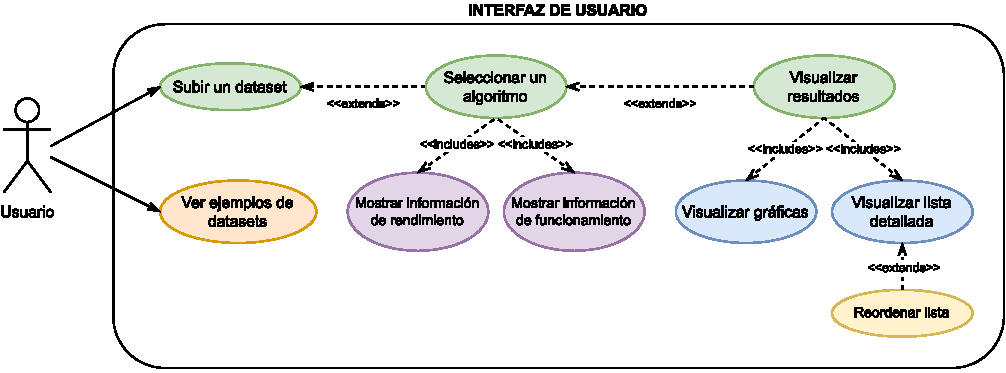
\includegraphics[width=\textwidth]{diagramas/usecases.pdf}
	\caption{Diagrama de casos de uso}
	\label{fig:casos_uso}
\end{figure}

\section{Requisitos no funcionales}
\label{sec:analisis_requisitos_no_funcionales}

Una vez definidas las funcionalidades que debe tener la aplicación, es necesario definir cuales van a ser sus requisitos
no funcionales, esto es, aquellos que están relacionados en cómo debe funcionar la aplicación. Para ello, se han tenido
en cuenta los aspectos recogidos en la Tabla \ref{tab:requisitos_no_funcionales}.

\bigskip
\begin{table}[hp!]
  \centering
  \rowcolors{2}{white}{udcgray!25}
  \begin{tabular}{c|p{9.6cm}}
		\rowcolor{udcpink!25}
		\small \textbf{Requisito} & \small \textbf{Descripción} \\\hline
		\small \textit{Usabilidad} & \small La aplicación debe ser fácil de usar, de forma que cualquier usuario pueda utilizarla sin
		necesidad de tener conocimientos previos sobre el perfilado de autores \\
		\small \textit{Escalabilidad} & \small La aplicación debe ser capaz de procesar datasets de cualquier tamaño, de forma que no
		exista un límite en el tamaño de los mismos \\
		\small \textit{Portabilidad} & \small La aplicación debe ser capaz de ejecutarse en cualquier sistema, de forma que
		los usuarios no tengan que preocuparse por el dispositivo que utilizan \\
  \end{tabular}
  \caption{Requisitos no funcionales}
  \label{tab:requisitos_no_funcionales}
\end{table}

\include{contenido/diseño}
\chapter{Implementación}
\label{chap:implementacion}

\lettrine{A} lo largo de este capítulo, se expondrán las decisiones de implementación más relevantes tomadas durante el desarrollo de la aplicación.
y se detallará la estructura de directorios que se ha seguido para organizar el código fuente del proyecto. Finalmente, se hablará
de la importancia del código abierto y de como contribuye a la innovación en el campo de la informática.

\section{Adaptación de los algoritmos}
\label{sec:adaptacion_algoritmos}

Dado que el código fuente de los algoritmos de perfilado seleccionados estaba disponible para su uso, fue necesario adaptarlo
para ofrecer una interfaz común a través de la cual se pudiese comunicar el resto de la aplicación.
Para ello se barajaron en un inicio dos aproximaciones diferentes. La primera de ellas pasaba
por implementar APIs sencillas en cada uno de los algoritmos, es decir, crear microservicios que se encargasen de recibir
las peticiones y devolver los resultados al \textit{backend}. La segunda aproximación consistía en adaptar el propio código
fuente para que cada algoritmo formase parte de una clase que implemente la interfaz mencionada en el diagrama de la Figura \ref{fig:clases_backend}
(\textit{ProfilingAlgorithm}). Finalmente, se optó por esta segunda opción ya que, a pesar de ser más compleja, permitía
una mayor integración con el resto de la aplicación y un mejor rendimiento debido a la eliminación de la latencia de red. Además,
podíamos aprovechar el hecho de que los algoritmos estaban programados en Python para utilizarlos directamente
en el \textit{backend} sin hacer uso de llamadas interlenguaje.

\bigskip
Sin embargo, esta decisión implicó comprender a muy bajo nivel como estaban implementados dichos algoritmos para realizar las modificaciones necesarias
e implementar nuevas funciones. Esta adaptación del código fue, en el caso del algoritmo de Grivas et al. \cite{grivas2015author},
bastante compleja, ya que conllevó sustituír librerías obsoletas, reimplementar funciones y resolver los cambios disruptivos (\textit{breaking changes} en inglés) que suponía
dar el salto desde la versión 2.7 de Python a la 3.10.

\section{Estructura del proyecto}
\label{sec:estructura_proyecto}

En relación a la estructura del proyecto, se ha optado por agrupar el código fuente de todo el sistema
bajo un mismo directorio, como se muestra en el diagrama de la Figura \ref{fig:estructura_proyecto},
dado que facilita en gran medida su portabilidad y su mantenimiento al tratarse de un proyecto relativamente
pequeño.

\bigskip
En primer lugar, situados en la raíz del proyecto, podemos diferenciar las carpetas principales que lo conforman, esto es,
\textit{backend}, \textit{fronted} y \textit{datasets}, así como dos archivos:

\begin{itemize}
	\item \textbf{\textit{README.md}}: Contiene un resumen en formato Markdown \cite{markdown} de lo que es la aplicación, de sus características y de la forma de ejecutarla.
	\item \textbf{\textit{docker-compose.yml}}: Es el archivo que almacena las configuraciones de los contenedores de Docker que se deben levantar para que el sistema funcione adecuadamente.
\end{itemize}

\bigskip
Continuando con el directorio \textit{backend}, distinguimos varias carpetas y archivos:

\begin{itemize}
	\item \textbf{\textit{requirements.txt}}: Contiene todas las dependencias de Python que necesita el \textit{backend} para funcionar.
	\item \textbf{\textit{Dockerfile}}: Es el archivo en el que se definen los pasos necesarios, es decir, los comandos a ejecutar en una
	      máquina recién instalada, para construir la imagen de Docker del \textit{backend}.
	\item \textbf{\textit{docker-compose.yml}}: A diferencia del situado en la raíz, este archivo contiene las configuraciones de los contenedores necesarios
	      para el correcto funcionamiento del entorno de desarrollo en el \textit{backend}.
	\item \textbf{\textit{/venv}}: Dado que el proyecto está creado haciendo uso de un entorno virtual para aislar las dependencias de Python, este directorio
	      contiene los archivos para su puesta en marcha.
	\item \textbf{\textit{/src}}: Aquí se almacena todo el código fuente del \textit{backend}, donde podemos encontrar las siguientes carpetas principales:
	      \begin{itemize}
		      \item \textbf{\textit{/application}}: Contiene los controladores y, en general, lo que se encarga de gestionar las comunicaciones exteriores con el sistema.
		      \item \textbf{\textit{/domain}}: Contiene las clases que conforman la capa de dominio, es decir, las entidades, los repositorios, los servicios, los algoritmos
		            y los conversores.
		      \item \textbf{\textit{/infraestructure}}: Contiene los repositorios de tecnologías concretas que implementan las interfaces definidas en la capa de dominio.
		      \item \textbf{\textit{/utils}}: Contiene clases de utilidad requeridas en diversas partes del sistema.
		      \item \textbf{\textit{main.py}}: Se corresponde con el punto de entrada de la aplicación.
	      \end{itemize}
\end{itemize}

\bigskip
Por otro lado, la estructura que sigue el \textit{frontend}, muy ligada al \textit{framework} de dearrollo NextJS, es la siguiente:

\begin{itemize}
	\item \textbf{\textit{package.json}}: En este archivo se almacenan todas las dependencias de NodeJS que requiere el \textit{frontend}.
	\item \textbf{\textit{next.config.js}}: La importancia de este archivo, más allá de contener las configuraciones básicas de NextJS, reside en la posibilidad
	      de definir un \textit{reverse proxy} capaz de redirigir las peticiones al \textit{backend} a la máquina local durante el desarrollo o a la máquina remota,
	      en este caso otro contenedor de Docker, en producción.
	\item \textbf{\textit{Dockerfile}}: Archivo análogo al presente en el directorio \textit{backend}, necesario para la construcción de la imagen del \textit{frontend}.
	\item \textbf{\textit{/src}}: Dentro de esta carpeta, nos encotramos la estructura típica de un proyecto en NextJS:
	      \begin{itemize}
		      \item \textbf{\textit{/components}}: Contiene los componentes que conforman las páginas de la aplicación.
		      \item \textbf{\textit{/model}}: Contiene las clases que representan las entidades del sistema en el \textit{frontend}.
		      \item \textbf{\textit{/pages}}: Contiene las páginas navegables de la aplicación, estructuradas en directorios según su ruta.
		      \item \textbf{\textit{/services}}: Contiene los servicios encargados de abstraer las peticiones que se realizan al \textit{backend}.
		      \item \textbf{\textit{/styles}}: Contiene las hojas de estilos globales de la aplicación.
		      \item \textbf{\textit{/utils}}: Contiene funciones de diversa utilidad en el proyecto.
	      \end{itemize}
\end{itemize}

\bigskip
Finalmente, el directorio \textit{datasets} se corresponde con el lugar donde se agrupan todas las colecciones que se han utilizado
para el entrenamiento y la validación de los modelos. Entre ellos se incluye una gran parte de \textit{datasets} ofrecidos por PAN \cite{pan} en las competiciones
de perfilado de autor que organiza, además de otras como la del movimiento \#BLM ofrecida en este trabajo y de la que se profundizará más en la Sección \ref{sec:casouso_dataset}.

\bigskip
\begin{figure}[H]
	\centering
	\begin{subfigure}[T]{0.5\textwidth}
		\begin{forest}
			for tree={
			font=\ttfamily\tiny,
			grow'=0,
			child anchor=west,
			parent anchor=south,
			inner xsep=10pt,
			anchor=west,
			calign=first,
			edge path={
					\noexpand\path [draw, \forestoption{edge}]
					(!u.south west) +(7.5pt,0) |- node[fill,inner sep=1.25pt] {} (.child anchor)\forestoption{edge label};
				},
			before typesetting nodes={
					if n=1
						{insert before={[,phantom]}}
						{}
				},
			fit=band,
			s sep=8pt,
			before computing xy={l=15pt},
			}
			[root, fill=gray!20
			[README.md, fill=gray!20]
			[docker-compose.yml, fill=gray!20]
			[/backend, for tree={fill=blue!20}
			[/src
			[/application]
			[/domain
			[/algorithms]
			[/converters]
			[/entities]
			[/repositories]
			[/services]
			]
			[/infraestructure]
			[/utils]
			[/main.py]
			]
			[/venv]
			[docker-compose.yml]
			[Dockerfile]
			[requirements.txt]
			]
			]
		\end{forest}
	\end{subfigure}%
	\begin{subfigure}[T]{0.5\textwidth}
		\begin{forest}
			for tree={
			font=\ttfamily\tiny,
			grow'=0,
			child anchor=west,
			parent anchor=south,
			inner xsep=10pt,
			anchor=west,
			calign=first,
			edge path={
					\noexpand\path [draw, \forestoption{edge}]
					(!u.south west) +(7.5pt,0) |- node[fill,inner sep=1.25pt] {} (.child anchor)\forestoption{edge label};
				},
			before typesetting nodes={
					if n=1
						{insert before={[,phantom]}}
						{}
				},
			fit=band,
			s sep=8pt,
			before computing xy={l=15pt},
			}
			[root, fill=gray!20
			[/frontend, for tree={fill=orange!20}
			[/src
			[/components]
			[/model]
			[/pages]
			[/services]
			[/styles]
			[/utils]
			]
			[Dockerfile]
			[package.json]
			[next.config.js]
			]
			[/datasets, for tree={fill=red!20}
				[/BLM20 - Reddit Collection]
				[/PAN13 - Author Profiling]
				[/PAN14 - Author Profiling]
				[/PAN15 - Author Profiling]
				[/PAN19 - Celebrity Profiling]
				[/PAN19 - Bots and Gender Profiling]
			]
			]
		\end{forest}
	\end{subfigure}
	\caption{Estructura de directorios del proyecto}
	\label{fig:estructura_proyecto}
\end{figure}

\section{Publicación del código fuente}
\label{sec:codigo_abierto}

Una vez explicado el funcionamiento a bajo nivel de la aplicación, es necesario valorar la forma de publicar y
distribuír el código fuente de la misma.

\bigskip
En este sentido, existen dos enfoques principales: el código abierto y el código privado.
El código privado (\textit{closed source} o \textit{propietary source} en inglés) es aquel que no está disponible para el público en general, es decir, que no se puede acceder a él ni
modificarlo, por lo que normalmente se asocia al mundo empresarial y a la venta de licencias para su uso.
Por otro lado, el código abierto (\textit{open source} en inglés) es aquel que
está disponible públicamente y puede ser modificado, utilizado y distribuído por cualquier persona en función
de la licencia bajo la que esté publicado. Normalmente, el código abierto se asocia con la filosofía del \textit{software} libre
y con la gratuidad de la aplicación, aunque esto no siempre es así.

\bigskip
En nuestro caso, creemos que la mejor forma de publicar el código fuente de la aplicación es hacerlo de forma abierta,
favoreciendo a una mejora continua de la misma por parte de la comunidad y a ofrecer la posibilidad de que cualquiera pueda
utilizarla y adaptarla a sus necesidades.

\bigskip
Sin embargo, para que esto sea posible, como se mencionó anteriormente, es necesario elegir una licencia bajo la cual publicarla. Así, existen licencias
como la GPL (\textit{General Public License} en inglés) \cite{gpl} que permiten a los usuarios hacer uso del código, modificarlo y distribuirlo
siempre y cuando se mantenga la misma licencia. Por otro lado, existen licencias como la MIT \cite{mitlicense} o la Apache \cite{apachelicense} que ofrecen una mayor libertad,
permitiendo incluso la utilización del código en proyectos privados. Por lo tanto, teniendo en cuenta que la filosofía de este proyecto es la de ofrecer una herramienta útil y gratuita a la mayor
cantidad de usuarios, sin importar si sus fines son comerciales o no, se ha optado por utilizar la licencia MIT. Asimismo, también se consideró la opción de publicar el código
bajo una doble licencia, pero se descartó por los complicaciones legales que suponía y por la confusión que podría generar.

\bigskip
En lo que respecta al lugar de publicación, se ha decidido hacer público el repositorio almacenado en GitHub \cite{github}, una de las
plataformas más populares para el alojamiento de proyectos de software con más de 100 millones de desarrolladores \cite{100milliongithub}.
Además, GitHub ofrece una gran cantidad de herramientas que facilitan el desarrollo colaborativo, como la posibilidad de crear \textit{issues} para
reportar errores o sugerir mejoras o la opción realizar \textit{pull requests} para proponer cambios en el código.

\bigskip
Por úlitmo, para que la comunidad pueda contribuir al proyecto de la mejor forma posible, se ha creado una guía de contribución
en la que se detallan los pasos a seguir para proponer cambios en el código, así como las normas de estilo que se deben cumplir.

\bigskip
Para acceder al repositorio, se puede hacer uso del siguiente enlace: \url{https://github.com/daavidrgz/ai-profiler}.

\chapter{Caso de uso: \#BLM}
\label{chap:casouso}
\chapter{Planificación y costes}
\label{chap:planificacion}
\chapter{Conclusiones}
\label{chap:conclusiones}

\lettrine{E}{n} este capítulo final se presentan las posibles mejoras que se podrían realizar en un futuro a la herramienta desarrollada,
así como las lecciones aprendidas durante el transcurso de este trabajo.


\section{Trabajo futuro}
\label{sec:trabajo_futuro}

Mirando a futuro, se pueden plantear diversas mejoras que podrían mejorar la aplicación y ampliar su alcance.

\bigskip
En primer lugar, el problema que suponen los conjuntos de datos desbalanceados y poco representativos estadísticamente, como se ha comprobado en el Capítulo \ref{chap:casouso},
es algo que perjudica en gran medida a los resultados obtenidos y limita los casos de uso de la aplicación a aquellos en los que se quieran predecir características
de autores similares a los utilizados para entrenar los modelos. Así, uno de los objetivos principales sería el de conseguir un mayor y más variado número de \textit{datasets}
con los que entrenar los modelos haciendo uso de los algoritmos previamente implementados.

\bigskip
En segundo lugar, se podría mejorar la experiencia de usuario ofreciendo más formas de especificar la fuente de textos para el perfilado.
Así, a mayores de un campo que permita la subida de un \textit{dataset} almacenado en local, se podría incluír un campo que permita la introducción
de un usuario de una red social como Twitter o Reddit, de forma que se puedan obtener los textos automáticamente y clasificar así a dicho usuario.

\bigskip
Por otro lado, a raíz de la aparición de los LLMs (\textit{Large Langauge Model} en inglés) como GPT-3 (Brown et al., 2020) \cite{brown2020language}
y, posteriormente, con modelos como GPT-4 en 2023, se ha visto un gran avance en las técnicas de \textit{Deep Learning}
y se ha demostrado el gran potencial que ofrecen estas herramientas para el procesado de lenguaje natural. Tal es así, que estos modelos
podrían ser utilizados en el campo del perfilado de autores. Sin embargo, debido a la gran cantidad de recursos
computacionales que actualmente requieren, en el caso de que su código haya sido liberado, o a la inversión de dinero que supondría su uso, en el caso
de que sea privado, irían en contra de los principios fundamentales de este trabajo: ofrecer una herramienta gratuita
y accesible a todo tipo de usuarios.

\section{Lecciones aprendidas}
\label{sec:lecciones_aprendidas}

El hecho de profundizar tanto en el campo del procesado del lenguaje natural y, más específicamente,
en las técnicas de perfilado automático de autores, supuso un gran reto tanto desde el punto de vista teórico como
desde el punto de vista de la propia investigación, a lo que se le suma la poca experiencia en un campo tan profundo. De esta forma, a lo largo del
proceso de investigación, se comprendieron las bases teóricas de técnicas como el TF-IDF o los n-gramas y se entendió a
bajo nivel el funcionamiento de los algoritmos que mejores resultados obtenían en las tareas analizadas.

\bigskip
Asimismo, ya que los objetivos del proyecto, más ambiciosos, no se quedaban en el terreno de la investigación
sino que buscaban implementar una aplicación completa con la información adquirida, el desarrollo implicó un trabajo
mucho más amplio, abordando diversas ramas de la informática. Desde el diseño y la implementación de una interfaz web gráfica,
pasando por la creación de un servidor web y el entrenamiento de modelos basados en algoritmos clásicos
de aprendizaje automático, hasta el seguimiento de metodologías de desarrollo ágiles como Scrum, conllevó
un gran esfuerzo junto a un aprendizaje continuo.

\bigskip
Más concretamente, se aprendió a desarrollar haciendo uso de Python en el \textit{backend} de la aplicación, consolidándose
como una opción ágil y fiable; se comprendió también la importancia de diseñar una buena interfaz
y de ofrecer una buena experiencia de usuario; y se profundizó más en el terreno del \textit{open source} y de las licencias
que, de alguna forma, promueven algo fundamental en nuestro campo.

\bigskip
Por último, destacar que se adquirieron conocimientos más allá de la informática tras realizar el análisis del caso de uso del fenómeno \#BLM,
uno de los movimientos sociales de mayor relevancia y complejidad en los últimos años. Además, esta tarea condujo
a poder conocer en mayor profundidad las redes sociales y las distribuciones demográficas
de los usuarios que las forman.

\section{Conclusiones finales}
\label{sec:conclusiones_finales}

\bigskip
Llegados a este punto, se puede decir que los objetivos establecidos al inicio del proyecto se han cumplido y que,
además, su desarrollo ha contribuido a poner en práctica los conocimientos adquiridos durante la carrera.
Asignaturas como Diseño Software, Internet y Sistemas Distribuidos, Aprendizaje Automático o Recuperación de Información,
han servido de fundamento para la consecución de dichos objetivos y han ayudado en gran medida al desarrollo de este proyecto.

\bigskip
En conclusión, a lo largo de este trabajo se ha demostrado que el perfilado automático de autor tiene la capacidad de posicionarse
como una herramienta muy útil para una gran cantidad de usuarios y que, partiendo de algoritmos clásicos y muy estudiados en el campo del aprendizaje automático,
se pueden obtener grandes resultados. De esta forma, se ha conseguido concluir un proyecto que, desde su nacimiento, buscaba
un punto de encuentro entre la investigación, el desarrollo y el análisis de datos, suponiendo, a mayores de un gran reto,
un gran crecimiento tanto personal como profesional.



%%%%%%%%%%%%%%%%%%%%%%%%%%%%%%%%%%%%%%%%
% Apéndices, glosarios e bibliografía  %
%%%%%%%%%%%%%%%%%%%%%%%%%%%%%%%%%%%%%%%%

\printglossary[type=\acronymtype,title=\nomeglosarioacronimos]
\printglossary[title=\nomeglosariotermos]

\bibliographystyle{IEEEtranN}
\bibliography{\bibconfig,bibliografia/bibliografia}
\clearpage

\end{document}

%%%%%%%%%%%%%%%%%%%%%%%%%%%%%%%%%%%%%%%%%%%%%%%%%%%%%%%%%%%%%%%%%%%%%%%%%%%%%%%%
